
%(BEGIN_QUESTION)
% Copyright 2011, Tony R. Kuphaldt, released under the Creative Commons Attribution License (v 1.0)
% This means you may do almost anything with this work of mine, so long as you give me proper credit

Identify suitable input terminals, proper modes, and necessary connecting wires to allow this National Instruments E-series data acquisition unit (DAQ) to sense the two voltage sources shown:

$$\includegraphics[width=15.5cm]{i01686x01.eps}$$

The available modes for the input channels are RSE, NRSE, and DIFF:

% No blank lines allowed between lines of an \halign structure!
% I use comments (%) instead, so that TeX doesn't choke.

$$\vbox{\offinterlineskip
\halign{\strut
\vrule \quad\hfil # \ \hfil & 
\vrule \quad\hfil # \ \hfil & 
\vrule \quad\hfil # \ \hfil & 
\vrule \quad\hfil # \ \hfil \vrule \cr
\noalign{\hrule}
%
% First row
{\bf Channel} & {\bf Mode} & {\bf First terminal} & {\bf Second terminal} \cr
%
\noalign{\hrule}
%
% Another row
0 &  &  &  \cr
%
\noalign{\hrule}
%
% Another row
1 &  &  &  \cr
%
\noalign{\hrule}
} % End of \halign 
}$$ % End of \vbox

\vfil 

\underbar{file i01686}
\eject
%(END_QUESTION)





%(BEGIN_ANSWER)

This is one possible solution:

$$\includegraphics[width=15.5cm]{i01686x02.eps}$$

% No blank lines allowed between lines of an \halign structure!
% I use comments (%) instead, so that TeX doesn't choke.

$$\vbox{\offinterlineskip
\halign{\strut
\vrule \quad\hfil # \ \hfil & 
\vrule \quad\hfil # \ \hfil & 
\vrule \quad\hfil # \ \hfil & 
\vrule \quad\hfil # \ \hfil \vrule \cr
\noalign{\hrule}
%
% First row
{\bf Channel} & {\bf Mode} & {\bf First terminal} & {\bf Second terminal} \cr
%
\noalign{\hrule}
%
% Another row
0 & RSE & AI0 & AI Gnd \cr
%
\noalign{\hrule}
%
% Another row
1 & NRSE & AI1 & AI Sense \cr
%
\noalign{\hrule}
} % End of \halign 
}$$ % End of \vbox


%(END_ANSWER)





%(BEGIN_NOTES)


%INDEX% Pictorial circuit review (analog signal wiring to data acquisition unit)

%(END_NOTES)

